% =====================================================================
% AI Academy -- National AI Center
% Software Engineering Final Project -- Defense Deck
% Team1 -- Topic 4: Async Research Assistant
%
% Build:  tectonic slides.tex     (or pdflatex slides.tex, twice)
% =====================================================================

\PassOptionsToPackage{dvipsnames}{xcolor}
\documentclass[aspectratio=169,11pt]{beamer}

% ===== CONFIGURATION =================================================
\newcommand{\teamname}{Team1}
\newcommand{\topicchoice}{Topic 4 -- Async Research Assistant}
\newcommand{\memberone}{Nurana Aliyeva}
\newcommand{\membertwo}{Elshan Shukurov}
\newcommand{\memberthree}{Ali Hasanli}
\newcommand{\memberfour}{Gasham Huseynli}
\newcommand{\repolink}{github.com/Nurana100/team1-ai-eng-research-assistant}
\newcommand{\defensedate}{19 September 2026}

\newcommand{\coursecode}{AI-ENG-110}
\newcommand{\coursename}{Software Engineering}
\newcommand{\institution}{AI Academy, National AI Center}
\newcommand{\semester}{Spring 2026}

% ===== PACKAGES ======================================================
\usepackage[T1]{fontenc}
\usepackage[utf8]{inputenc}
\usepackage{xcolor}
\usepackage{tabularx}
\usepackage{booktabs}
\usepackage{listings}
\usepackage{tikz}
\usetikzlibrary{shapes.geometric,arrows.meta,positioning,fit,backgrounds}

\definecolor{accent2}{HTML}{8B0000}

% ===== THEME =========================================================
\usetheme{default}
\usefonttheme{professionalfonts}
\setbeamertemplate{navigation symbols}{}

\definecolor{accent}{HTML}{0B3D91}
\definecolor{soft}{HTML}{F2F4F8}
\definecolor{ok}{HTML}{166534}
\definecolor{warn}{HTML}{B45309}

\setbeamercolor{title}{fg=accent}
\setbeamercolor{frametitle}{fg=accent}
\setbeamercolor{section in head/foot}{bg=accent,fg=white}
\setbeamercolor{itemize item}{fg=accent}
\setbeamercolor{itemize subitem}{fg=accent}
\setbeamercolor{enumerate item}{fg=accent}
\setbeamercolor{block title}{bg=accent,fg=white}
\setbeamercolor{block body}{bg=soft,fg=black}

\setbeamerfont{title}{size=\Large,series=\bfseries}
\setbeamerfont{frametitle}{size=\large,series=\bfseries}
\setbeamerfont{footline}{size=\tiny}

\setbeamertemplate{footline}{%
  \leavevmode%
  \hbox to\paperwidth{\hspace*{2ex}\tiny\textit{\teamname{} -- Topic 4}\hfill%
  \tiny\textit{\coursecode{} -- \semester{}}\hfill%
  \tiny\insertframenumber/\inserttotalframenumber\hspace*{2ex}}%
  \vskip2pt%
}

\definecolor{codegreen}{rgb}{0,0.55,0}
\definecolor{codepurple}{rgb}{0.55,0,0.78}
\lstdefinestyle{python}{
  language=Python,
  backgroundcolor=\color{soft},
  commentstyle=\color{codegreen},
  keywordstyle=\color{accent},
  stringstyle=\color{codepurple},
  basicstyle=\ttfamily\scriptsize,
  breaklines=true,
  frame=single,
  framerule=0.4pt,
  rulecolor=\color{black!30},
}
\lstdefinestyle{shell}{
  backgroundcolor=\color{soft},
  basicstyle=\ttfamily\scriptsize,
  breaklines=true,
  frame=single,
  framerule=0.4pt,
  rulecolor=\color{black!30},
}

% =====================================================================
\begin{document}

% ========== 1: TITLE =================================================
{%
\setbeamertemplate{footline}{}
\begin{frame}[plain]
  \begin{center}
    \vspace{0.5cm}
    {\small \textsc{\institution}}\\[0.2em]
    {\small \textsc{\coursecode{} -- \coursename{} -- \semester{}}}\\[1.0em]
    \rule{0.7\textwidth}{0.6pt}\\[0.4em]
    {\LARGE\bfseries\color{accent} \topicchoice}\\[0.4em]
    \rule{0.7\textwidth}{0.6pt}\\[1.0em]
    {\large \teamname}\\[0.5em]
    {\normalsize \memberone\quad\textbullet\quad\membertwo\quad\textbullet\quad\memberthree\quad\textbullet\quad\memberfour}\\[0.8cm]
    {\footnotesize\itshape Final Project Defense -- \defensedate}\\[0.4em]
    {\footnotesize\texttt{\repolink}\quad\textbullet\quad tag \texttt{v1.0-final}}
  \end{center}
\end{frame}
}

% ========== 2: PROBLEM ===============================================
\begin{frame}{The problem in one sentence}
  \begin{block}{What the system does}
    A user asks one natural-language research question; we fan out to Wikipedia, arXiv and web
    search \emph{at the same time} and return a single synthesized answer in which every claim
    carries a citation index pointing at a real URL.
  \end{block}

  \vspace{0.2em}
  \begin{columns}[T,onlytextwidth]
  \column{0.47\textwidth}
  \textbf{Inputs}
  \begin{itemize}\setlength\itemsep{0.15em}
    \item a question, $\le 500$ characters
    \item optional source filter \texttt{wiki,arxiv,web}
    \item \texttt{.env}: provider + keys
  \end{itemize}

  \column{0.50\textwidth}
  \textbf{Outputs}
  \begin{itemize}\setlength\itemsep{0.15em}
    \item cited prose answer + resolved source list
    \item one row in SQLite (question, answer, sources, UTC timestamp)
  \end{itemize}
  \end{columns}

  \vspace{0.5em}
  \textbf{Entry point:} one CLI --- \texttt{python -m src.cli ask "<question>"}\\
  \textbf{Stack:} Gemini \texttt{gemini-3.6-flash} for synthesis, DuckDuckGo for web search
  (no key needed)

  \vspace{0.3em}
  {\footnotesize\textit{Not built, deliberately: no HTTP API, no cross-question batch mode.}}
\end{frame}

% ========== 3: ARCHITECTURE ==========================================
\begin{frame}{Architecture --- one arrow crosses the \texttt{ai/} boundary}
  \vspace{-0.2em}
  \begin{center}
  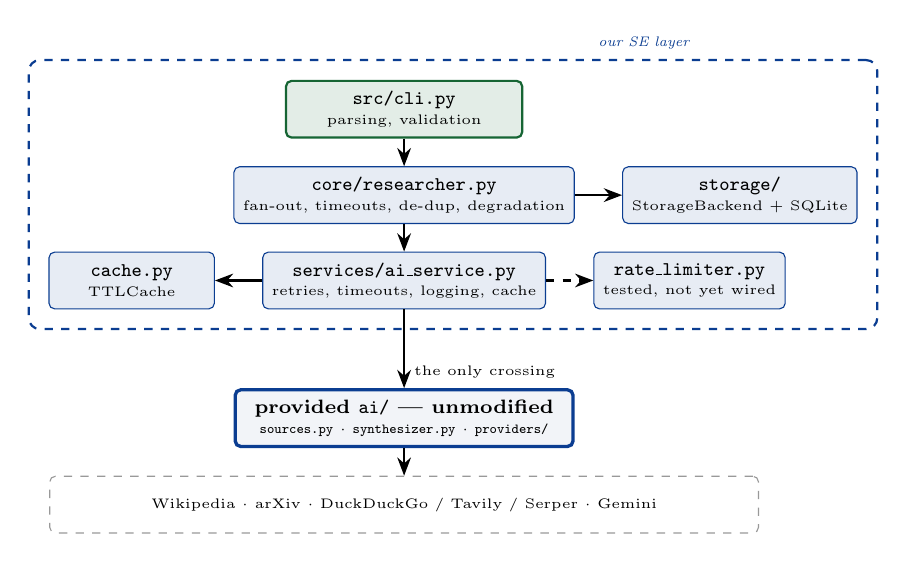
\begin{tikzpicture}[
    node distance=3.5mm and 6mm,
    box/.style={draw,rounded corners=2pt,minimum width=3.0cm,minimum height=0.72cm,align=center,font=\scriptsize},
    entry/.style={box,fill=ok!12,draw=ok,thick},
    sebox/.style={box,fill=accent!10,draw=accent},
    aibox/.style={box,fill=soft,draw=accent,very thick,inner xsep=7pt},
    ext/.style={box,fill=white,draw=black!40,dashed,font=\scriptsize},
    arrow/.style={-Stealth,thick}
  ]
    \node[entry] (cli) {\texttt{src/cli.py}\\[-1pt]{\tiny parsing, validation}};
    \node[sebox,below=of cli] (core) {\texttt{core/researcher.py}\\[-1pt]{\tiny fan-out, timeouts, de-dup, degradation}};
    \node[sebox,below=of core] (svc) {\texttt{services/ai\_service.py}\\[-1pt]{\tiny retries, timeouts, logging, cache}};
    \node[sebox,left=of svc,minimum width=2.1cm] (cache) {\texttt{cache.py}\\[-1pt]{\tiny TTLCache}};
    \node[sebox,right=of svc,minimum width=2.3cm] (rl) {\texttt{rate\_limiter.py}\\[-1pt]{\tiny tested, not yet wired}};
    \node[sebox,right=of core,minimum width=2.3cm] (store) {\texttt{storage/}\\[-1pt]{\tiny StorageBackend + SQLite}};
    \node[aibox,below=10mm of svc] (ai) {\textbf{provided \texttt{ai/} --- unmodified}\\[-1pt]{\tiny \texttt{sources.py} $\cdot$ \texttt{synthesizer.py} $\cdot$ \texttt{providers/}}};
    \node[ext,below=3.5mm of ai,minimum width=9cm] (net) {\tiny Wikipedia $\cdot$ arXiv $\cdot$ DuckDuckGo / Tavily / Serper $\cdot$ Gemini};

    \draw[arrow] (cli) -- (core);
    \draw[arrow] (core) -- (svc);
    \draw[arrow] (core) -- (store);
    \draw[arrow] (svc) -- (cache);
    \draw[arrow,dashed] (svc) -- (rl);
    \draw[arrow] (svc) -- node[right,font=\tiny,pos=0.8] {the only crossing} (ai);
    \draw[arrow] (ai) -- (net);

    \begin{scope}[on background layer]
      \node[draw=accent,dashed,thick,rounded corners,fit=(cli)(core)(svc)(cache)(rl)(store),
            inner sep=2.5mm,label={[font=\tiny\itshape,accent]above right:our SE layer}] {};
    \end{scope}
  \end{tikzpicture}
  \end{center}

  \vspace{-0.6em}
  {\footnotesize
  \textbf{Why it matters:} retries, timeouts, logging and caching are cross-cutting ---
  one file to change to add another. Swapping Gemini $\to$ Anthropic $\to$ OpenAI changes
  \textbf{zero source files}, two lines in \texttt{.env}.}
\end{frame}

% ========== 4: DESIGN DECISIONS ======================================
\begin{frame}{Three design decisions we can defend}
  \begin{enumerate}\setlength\itemsep{0.55em}
    \item \textbf{asyncio, not threads.}\\
      {\small The provided \texttt{ai/} fetchers are already coroutines over one shared
      \texttt{httpx.AsyncClient}; a thread pool would need an event loop per thread and throw
      away the connection pool. Rejected: \texttt{ThreadPoolExecutor} (per-source timeouts are
      awkward --- a blocked thread cannot be cancelled), \texttt{ProcessPoolExecutor} (no CPU work).}
    \item \textbf{One service class as the only seam over \texttt{ai/}.}\\
      {\small Every \texttt{ai.*} call goes through \texttt{AIService}, so retry policy, timeout,
      structured log and cache live in exactly one file. Trade-off accepted: that file is a
      chokepoint, and its coverage looks low because the uncovered lines are the provided
      functions themselves.}
    \item \textbf{\texttt{StorageBackend} as an ABC, not a \texttt{Protocol}.}\\
      {\small We want the failure at construction time: a half-finished \texttt{PostgresStorage}
      must refuse to instantiate, not explode later at the call site. We assert exactly that in
      \texttt{test\_abstract\_backend\_cannot\_be\_instantiated}.}
  \end{enumerate}
\end{frame}

% ========== 5: CONCURRENCY / BENCHMARK ===============================
\begin{frame}{Concurrency: the benchmark}
  \textbf{Live measurement: 3 sources (Wikipedia, arXiv, DuckDuckGo), 3 runs.}

  \vspace{0.3em}
  \begin{center}\footnotesize
  \begin{tabular}{lccc}
    \toprule
    \textbf{Run} & \textbf{Sequential} & \textbf{Concurrent} & \textbf{Speedup} \\
    \midrule
    1 & 1.29\,s & 0.71\,s & $1.82\times$ \\
    2 & 1.12\,s & 0.34\,s & $3.29\times$ \\
    3 & 1.16\,s & 0.65\,s & $1.78\times$ \\
    \midrule
    \textbf{Mean} & \textbf{1.19\,s} & \textbf{0.57\,s} & $\mathbf{2.10\times}$ \\
    \bottomrule
  \end{tabular}
  \end{center}

  \vspace{0.2em}
  {\small
  \textbf{Ceiling $\approx 2.7\times$; measured mean $2.10\times$.} For a fan-out the limit is not
  $N$ but $\sum t_i / \max t_i$ --- total serial time over the slowest leg
  ($1.20 / 0.45\,\mathrm{s}$). Run~2 exceeded the ceiling, which we treat as a warm-connection
  artifact of our harness (sequential pass runs first), not as a result.

  \smallskip
  \textbf{The bottleneck is width, not our code.} Three sources is not a wide fan-out; batching
  questions into one \texttt{gather} is the change that would move the curve. Next step for the
  harness: interleave the two modes and discard a warm-up round.}
\end{frame}

% ========== 6: ROBUSTNESS ============================================
\begin{frame}{Robustness: a failure we did not plan}
  \textbf{Scenario.} During an earlier benchmark run, Wikipedia started answering
  \texttt{403 Forbidden} to \emph{every} request --- about 30 requests in ten seconds.

  \vspace{0.35em}
  \begin{columns}[T,onlytextwidth]
  \column{0.49\textwidth}
  \textbf{What the system did}
  \begin{itemize}\setlength\itemsep{0.2em}
    \item {\small \texttt{gather(..., return\_exceptions=True)} kept the exception out of the caller}
    \item {\small \texttt{researcher.py} logged \texttt{WARNING} and skipped the dead source}
    \item {\small User got a normal, correctly-cited \textbf{arXiv-only} answer --- no traceback}
  \end{itemize}

  \column{0.49\textwidth}
  \textbf{What we expected vs.\ found}
  \begin{itemize}\setlength\itemsep{0.2em}
    \item {\small Expected the documented missing-\texttt{User-Agent} \texttt{403}}
    \item {\small Replayed the \emph{same} header 0.5\,s apart $\to$ \texttt{200} every time}
    \item {\small Real cause: \textbf{our own request rate}}
  \end{itemize}
  \end{columns}

  \vspace{0.4em}
  \begin{block}{What the experiment established}
    \small The header is necessary but not sufficient --- what Wikimedia rejected was one identity
    making thirty rapid requests. A rate condition, not an authentication one: the fix is a per-source minimum interval (our limiter exists, not yet wired in), not a header.
  \end{block}

\end{frame}

% ========== 7: CLI, CACHE, DOCKER ====================================
\begin{frame}{CLI, cache and Docker}
  \begin{columns}[T,onlytextwidth]
  \column{0.49\textwidth}
  \textbf{CLI} --- \texttt{src/cli.py}
  \begin{itemize}\setlength\itemsep{0.15em}
    \item {\small \texttt{python -m src.cli ask "<question>"} starts the async pipeline}
    \item {\small options: \texttt{-{}-sources} to pick sources, \texttt{-{}-no-cache} to skip the cache}
  \end{itemize}

  \vspace{0.3em}
  \textbf{TTL cache} --- \texttt{services/cache.py}
  \begin{itemize}\setlength\itemsep{0.15em}
    \item {\small TTL = time to live: a repeated question is answered from memory, with no new API call}
    \item {\small key = source name + lower-cased, trimmed question, so wiki and arXiv stay separate}
    \item {\small wired into \texttt{AIService} for wiki, arXiv and web}
  \end{itemize}

  \column{0.49\textwidth}
  \textbf{Tests}
  \begin{itemize}\setlength\itemsep{0.15em}
    \item {\small \texttt{tests/test\_cache.py}: store and read, expiry, normalisation, per-source keys}
    \item {\small \texttt{tests/test\_researcher.py}: success, partial failure, total failure, 3 sources in parallel}
  \end{itemize}

  \vspace{0.3em}
  \textbf{Docker and demo runner}
  \begin{itemize}\setlength\itemsep{0.15em}
    \item {\small \texttt{Dockerfile}: same Python environment, runs as a non-root user}
    \item {\small \texttt{scripts/run\_demo.py}: loads the 5 prepared questions and runs the pipeline for each}
  \end{itemize}
  \end{columns}
\end{frame}

% ========== 8: DEMO ==================================================
\begin{frame}[fragile]{Demo}
  \begin{block}{What we will run}
    One live question end to end, then the same question with arXiv excluded to show a source-filtered run,
    then an empty question to show a clean validation error.
  \end{block}

  \vspace{0.3em}
\begin{lstlisting}[style=shell]
$ python -m src.cli ask "Quantum Entanglement"
$ python -m src.cli ask "Quantum Entanglement" --sources wiki,web
$ python -m src.cli ask ""
\end{lstlisting}

  \vspace{0.2em}
  {\small
  \begin{itemize}\setlength\itemsep{0.2em}
    \item Every sentence in the answer carries a \texttt{[n]} index that resolves to a printed URL ---
      no uncited prose.
    \item A dead source gives a shorter source list, not a crash; bad input gives one
      \texttt{Error:} line, not a traceback.
  \end{itemize}}

  \vspace{0.2em}
  {\footnotesize\itshape Backup: \texttt{artefacts/demo\_run\_all.txt} holds a captured five-question
  run if the network or the LLM quota fails.}
\end{frame}

% ========== 8: TESTING ===============================================
\begin{frame}{Offline tests and SQLite storage}
  \begin{columns}[T,onlytextwidth]
  \column{0.52\textwidth}
  \textbf{Coverage \& shape}
  \begin{itemize}\setlength\itemsep{0.25em}
    \item {\small Coverage of \texttt{src/}: \textbf{76\%} (required $\ge 60\%$)}
    \item {\small Provided \texttt{ai/} smoke tests: \textcolor{ok}{\textbf{16/16 passing}}, \texttt{ai/} unmodified}
    \item {\small \textbf{51 tests}, 35 ours + 16 provided, in about 5\,s}
    \item {\small \textbf{Fully offline, enforced:} \texttt{MockTransport} raises on any outbound
      request; an autouse fixture deletes all five provider keys}
  \end{itemize}

  \column{0.46\textwidth}
  \textbf{Three worth calling out}
  \begin{itemize}\setlength\itemsep{0.25em}
    \item {\small \textbf{Happy path:} the stub delegates to the \emph{real} \texttt{synthesize},
      so citation numbering is genuine}
    \item {\small \textbf{Concurrency:} one source raises, the other two still come back}
    \item {\small \textbf{Error path:} storage tests caught a leaked SQLite connection and an
      unchecked \texttt{lastrowid}}
  \end{itemize}
  \end{columns}

  \vspace{0.5em}
  \begin{block}{SQLite storage --- \texttt{storage/repository.py}}
    \small \texttt{StorageBackend} ABC (save, get by ID, list recent) $\to$ \texttt{SQLiteStorage}: question,
    answer, sources as JSON, UTC time. It creates missing folders, closes every connection and checks the
    row id; database files are git-ignored. Test stubs live in \texttt{tests/conftest.py}.
  \end{block}
\end{frame}

% ========== 10: CONFIG, VALIDATION, INTEGRATION ======================
\begin{frame}{Config, validation and integration}
  \begin{columns}[T,onlytextwidth]
  \column{0.49\textwidth}
  \textbf{Configuration} --- \texttt{src/config.py}
  \begin{itemize}\setlength\itemsep{0.15em}
    \item {\small Pydantic Settings: typed provider, model, keys, log level, TTL, max parallel}
    \item {\small from environment or local \texttt{.env}; no keys in code}
  \end{itemize}

  \vspace{0.25em}
  \textbf{Input validation} --- CLI
  \begin{itemize}\setlength\itemsep{0.15em}
    \item {\small rejects empty or 500+ character questions, unknown or empty source lists}
  \end{itemize}

  \vspace{0.25em}
  \textbf{Rate limiter} --- \texttt{services/rate\_limiter.py}
  \begin{itemize}\setlength\itemsep{0.15em}
    \item {\small per-source minimum interval; tested, \emph{not yet wired} into \texttt{AIService}}
  \end{itemize}

  \column{0.49\textwidth}
  \textbf{Checks}
  \begin{itemize}\setlength\itemsep{0.15em}
    \item {\small \texttt{tests/test\_cli.py} and \texttt{tests/test\_config.py}}
    \item {\small mypy report + \texttt{docs/security\_check.md}: no TODOs, no hard-coded keys}
  \end{itemize}

  \vspace{0.25em}
  \textbf{Storage integration}
  \begin{itemize}\setlength\itemsep{0.15em}
    \item {\small CLI creates \texttt{SQLiteStorage}, passes it to \texttt{run\_research\_pipeline}}
    \item {\small saves question, answer, sources, UTC time; a test reads it back}
  \end{itemize}
  \end{columns}

  \vspace{0.4em}
  {\small\textbf{Final state:} storage wiring merged with the latest \texttt{main}, conflicts resolved, suite re-run --- \textbf{51 tests pass}.}
\end{frame}

% ========== 11: LIMITATIONS ==========================================
\begin{frame}{Limitations \& what we would do next}
  \small
  \textbf{Where the system is bounded today}
  \begin{itemize}\setlength\itemsep{0.15em}
    \item \textbf{Wikipedia's opensearch does not answer questions.} ``What is photosynthesis and
      what are its main stages?'' $\to$ 0 hits; ``photosynthesis'' $\to$ 3. The demo maps each
      known question to a keyword; a product needs query rewriting.
    \item \textbf{The fan-out is only three wide.} The ceiling is $\sum t_i / \max t_i$, so it
      stays below $3\times$ until batch mode widens it --- what \texttt{MAX\_PARALLEL} bounds.
    \item \textbf{The cache is per-process.} Right for a long-running caller; a one-shot CLI run
      starts cold. Persisting it into the SQLite file we already write closes that.
    \item \textbf{No provider failover, no answer-level validation.} A fluent answer that misreads
      its own citation goes undetected --- a research problem, not a weekend one.
    \item \textbf{SQLite is single-writer.} The \texttt{StorageBackend} ABC exists so Postgres can
      be dropped in without touching a caller.
  \end{itemize}

  \vspace{0.3em}
  \textbf{Given another week}, in priority order
  \begin{enumerate}\setlength\itemsep{0.1em}
    \item Batch mode with a real semaphore bound --- a workload wide enough to show the design.
    \item Wire in the rate limiter; query rewriting; persisted cache; CI (\texttt{pytest} + \texttt{mypy}).
  \end{enumerate}
\end{frame}

% ========== 10: CONTRIBUTIONS ========================================
\begin{frame}{Team contributions}
  \begin{center}\footnotesize
  \begin{tabularx}{\linewidth}{lXcc}
    \toprule
    \textbf{Member} & \textbf{Primary ownership} & \textbf{Commits} & \textbf{Share} \\
    \midrule
    \memberone   & CLI, pipeline orchestration, \texttt{AIService}, docs & 21 & 29.2\% \\
    \membertwo   & Offline test infrastructure, storage layer, config & 19 & 26.4\% \\
    \memberthree & first async CLI, \texttt{TTLCache} + wiring, Dockerfile, researcher tests & 19 & 26.4\% \\
    \memberfour  & Rate limiter, CLI validation + tests, security audit & 13 & 18.1\% \\
    \midrule
    \textbf{Total} & & \textbf{72} & \textbf{100\%} \\
    \bottomrule
  \end{tabularx}
  \end{center}

  \vspace{0.2em}
  \begin{block}{We can all answer}
    \small Every change reached \texttt{main} through a reviewed pull request. Pick a file --- we
    will walk through it.
  \end{block}

  \vspace{0.1em}
  {\footnotesize\textbf{AI tool use:} Claude drafted the test stubs, the tenacity decorator shape,
  the storage ABC and the benchmark script; we narrowed the retryable exception set, added \texttt{reraise=True}, and
  fixed two real defects in the storage draft. Per-module disclosure in report \S9.}
\end{frame}

% ========== 11: Q&A ==================================================
{%
\setbeamertemplate{footline}{}
\begin{frame}[plain]
  \begin{center}
    \vspace{0.8cm}
    {\Huge\bfseries\color{accent} Questions?}\\[1.0em]
    \rule{0.5\textwidth}{0.6pt}\\[1.0em]
    {\large \teamname{} -- \topicchoice}\\[0.5em]
    {\normalsize \texttt{\repolink}}\\[0.3em]
    {\footnotesize tag \texttt{v1.0-final}}\\[0.9cm]
    {\footnotesize\itshape ``We can walk through any file in the repo.''}
  \end{center}
\end{frame}
}

\end{document}
